\begin{figure}[t!]
    
    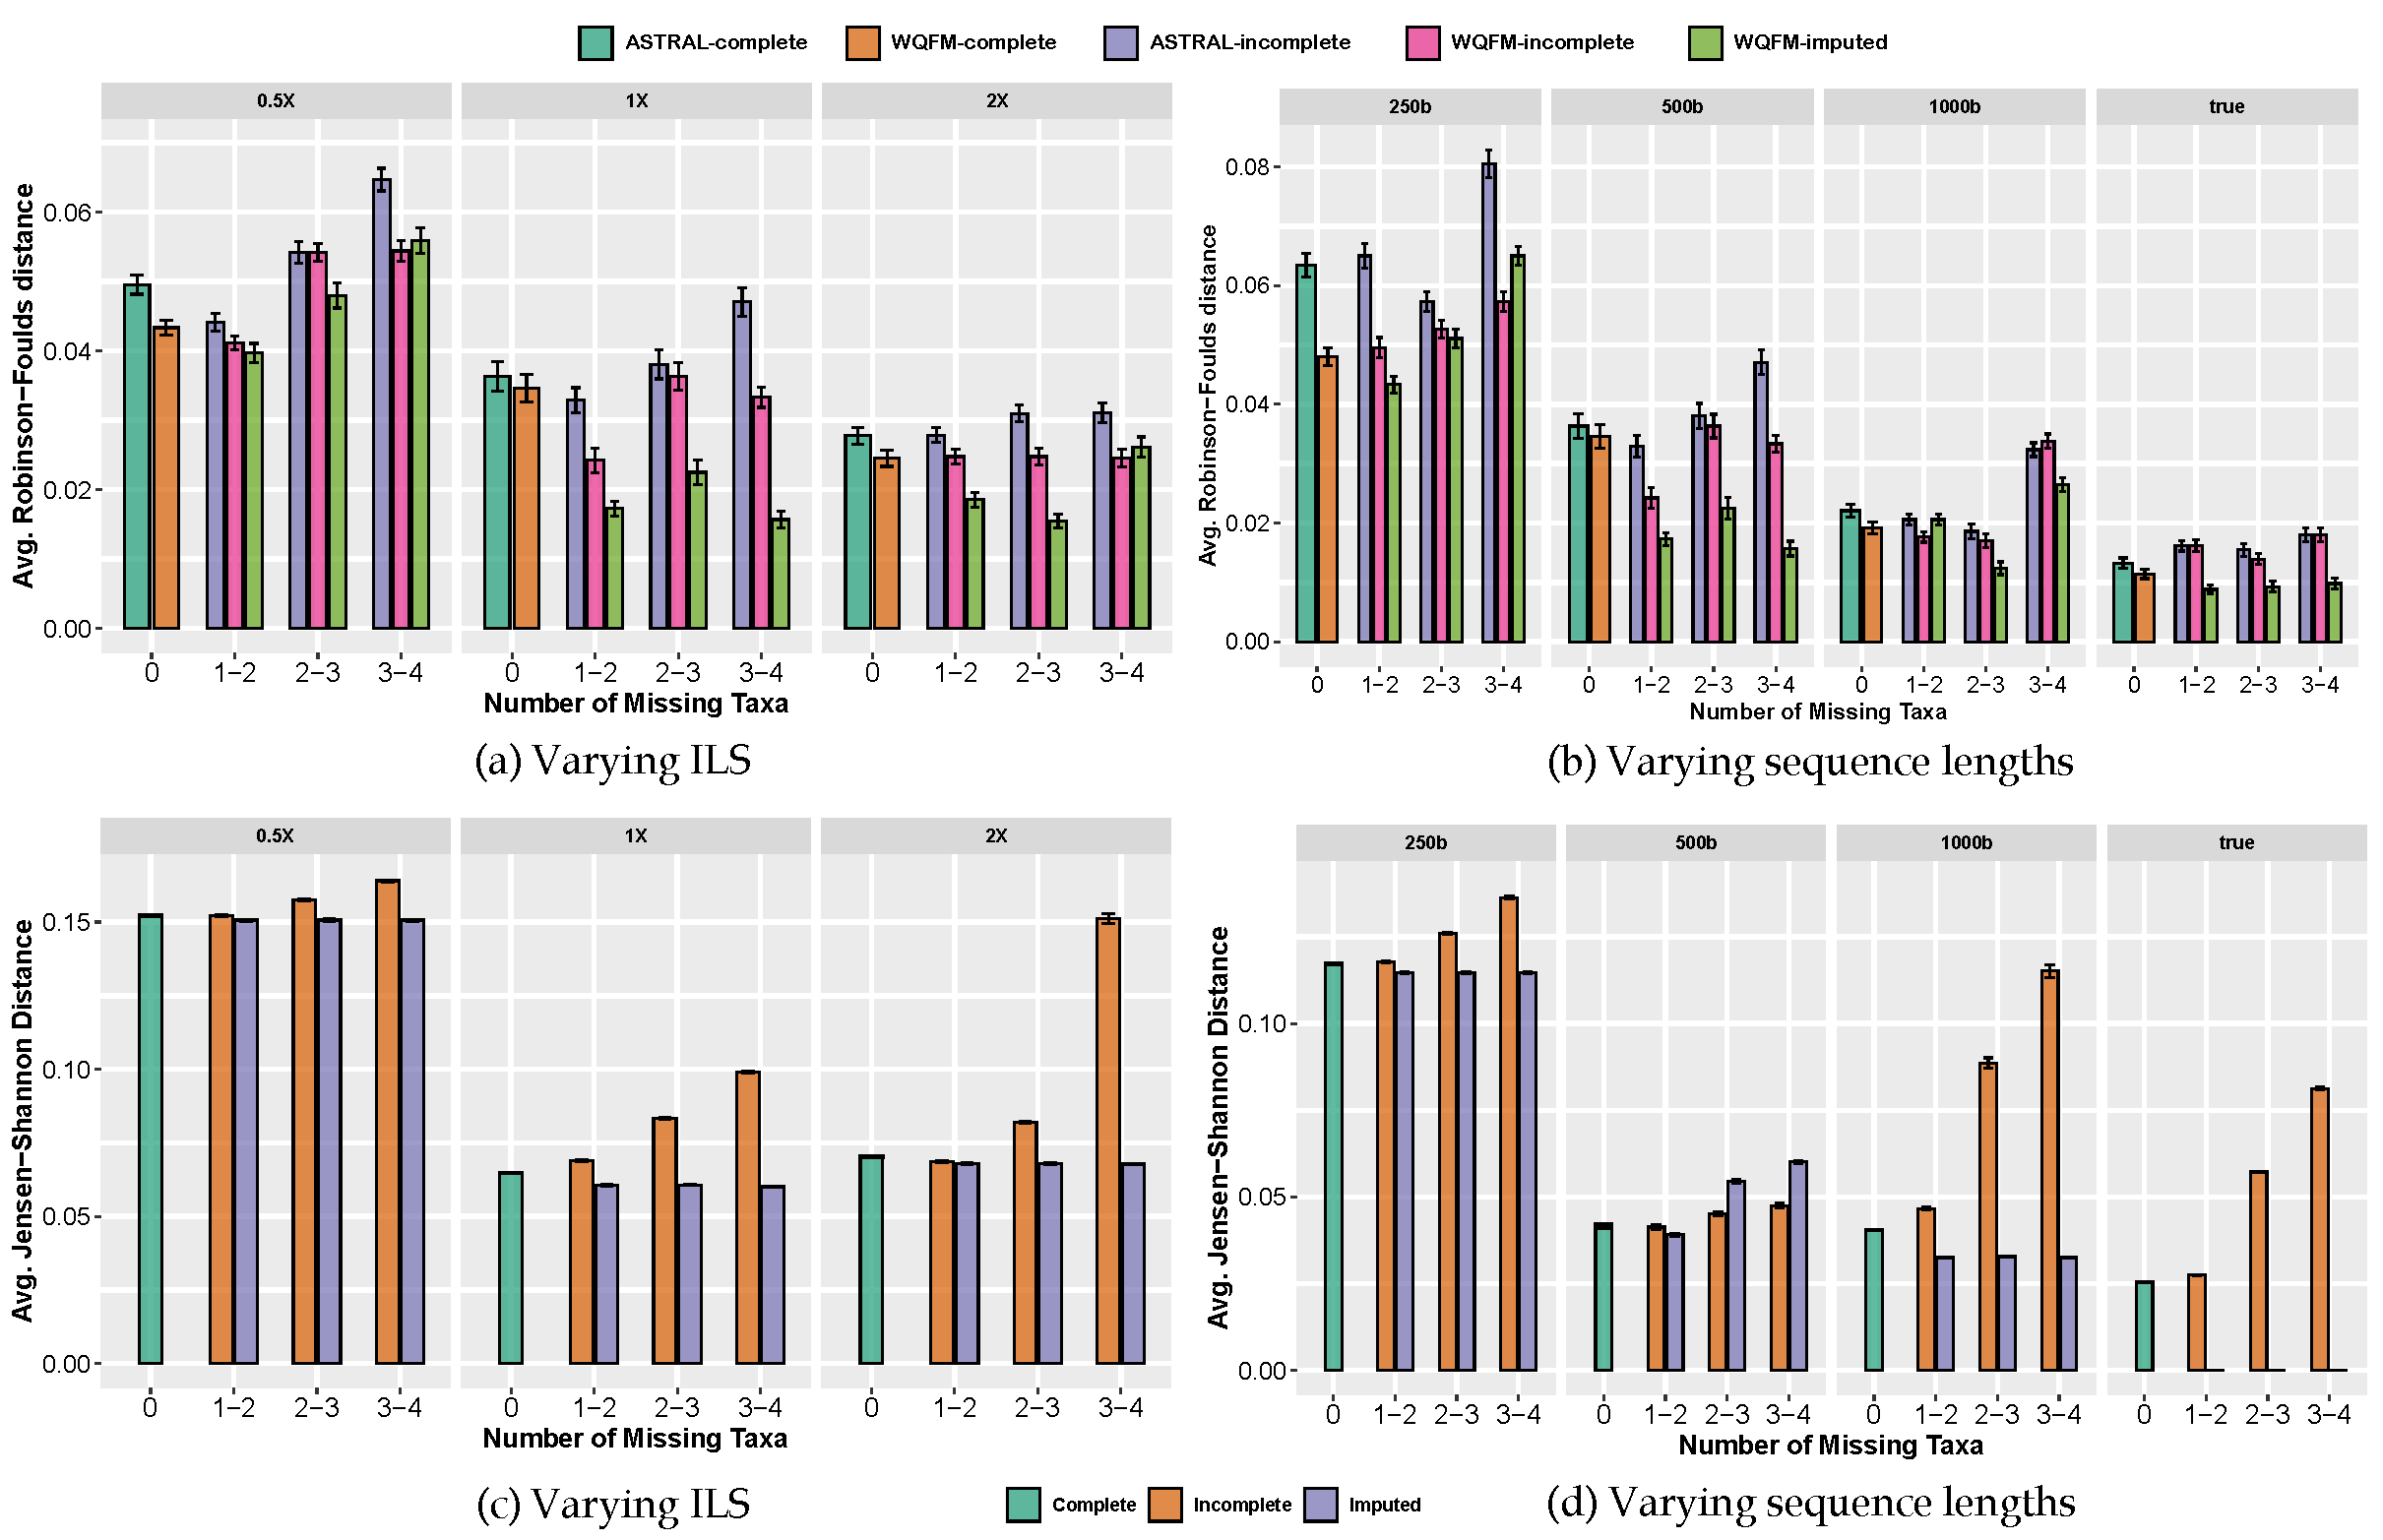
\includegraphics[width=\linewidth]{figures/37-taxon-combined.pdf}
    \caption{Results on 37-taxon dataset. (a)-(b) We show the average RF rates with standard errors over 20 replicates. (a) The level of ILS was varied from 0.5X (highest) to 2X (lowest) amount, keeping the sequence length fixed at 500bp and the number of genes at 200.
    (b) The sequence length was varied from 250bp to 1500bp, keeping the number of genes fixed at 200, and ILS at 1X (moderate ILS). We also analyzed the true gene trees. (c)-(d) Jansen-Shannon divergence between true quartet distributions and complete, incomplete and imputed quartet distributions.
    %(b) The number of genes was varied from 100 to 400, with 500bp sequence length and moderate (1X) ILS.
    }
    \label{fig:RF_Rates_37_Taxon}
    \end{figure}



In the simulated mammalian data, we explored the impact of varying numbers of genes (25 - 800), varying amounts of gene tree estimation error (i.e., the amount of phylogenetic signal by varying the sequence length for the markers: 250bp - 1500bp). We also investigated three levels of ILS (shorter branches increases ILS) by multiplying or dividing all internal branch lengths in the model species tree by two -- producing three model conditions that are referred to as 1X (moderate ILS), 0.5X (high ILS) and 2X (low ILS). For each model condition, we varied the taxa removal rate from $\sim$2\% to $\sim$10\%, resulting in 6 - 25\% missing quartets. Because the number of quartets grows exponentially with the number of taxa, even with 25\% missing quartets, the 37-taxon dataset contained a substantial number %($\sim$699300 - $\sim$3341384) 
($\sim$7,00,000 - $\sim$33,00,000) of missing quartets.

Fig.~\ref{fig:RF_Rates_37_Taxon}(a) shows the RF rates of various methods on varying ILS levels (0.5X, 1X, 2X) with 200 genes and a fixed sequence length (500 bp). As expected, species tree error rates of various methods increased as ILS level increased. Similar to 15-taxon dataset, wQFM is better than ASTRAL (both on complete and incomplete datasets), and wQFM-imputed is consistently better than wQFM-incomplete. Remarkably, for moderate (1X) to low ILS (2X) datasets, wQFM-imputed is substantially better than ASTRAL-complete and wQFM-complete (except for 3-4 taxa removal rate on 2X model condition).
On the high-ILS dataset (0.5X), wQFM-imputed is better than wQFM-incomplete and ASTRAL-incomplete. Moreover, for small amount of missing taxa (1-2), wQFM-imputed is even better than ASTRAL-complete and wQFM-complete.  % -- suggesting that QT-GILD not only effectively imputed the missing quartets but it corrects for estimation error as well.

RF rates on varying gene tree estimation error (controlled by sequence length; 500-1500 bp) are shown in  Figs.~\ref{fig:RF_Rates_37_Taxon} (b). All methods showed improved accuracy with increasing sequence lengths, and best results were obtained on true gene trees. These results clearly show that wQFM-imputed is better than wQFM-incomplete and ASTRAL-complete and, in many cases, it is even better than wQFM-complete and ASTRAL-complete. Similar to 15-taxon dataset, we investigated the divergence of various quartet distributions from true quartet distributions (see Fig.~\ref{fig:RF_Rates_37_Taxon}(c)-(d)) and the quartet scores of different estimated species trees with respect to both estimated and true gene trees (see Appendix~\ref{app:37-taxon}) and observed similar trends, supporting our claim that QT-GILD effectively imputes missing data and accounts for gene tree estimation error while imputing the missing quartets.
%Performance on varying gene tree estimation error (controlled by sequence length; 500- 1500 bp) is shown in Fig.~\ref{fig:RF_Rates_37_Taxon_Gene_variation}. We also analyzed the model condition with true gene trees (i.e., no estimation error). \add{Add the description once the figure is added.}


% \begin{figure}[H]
%     \centering
%     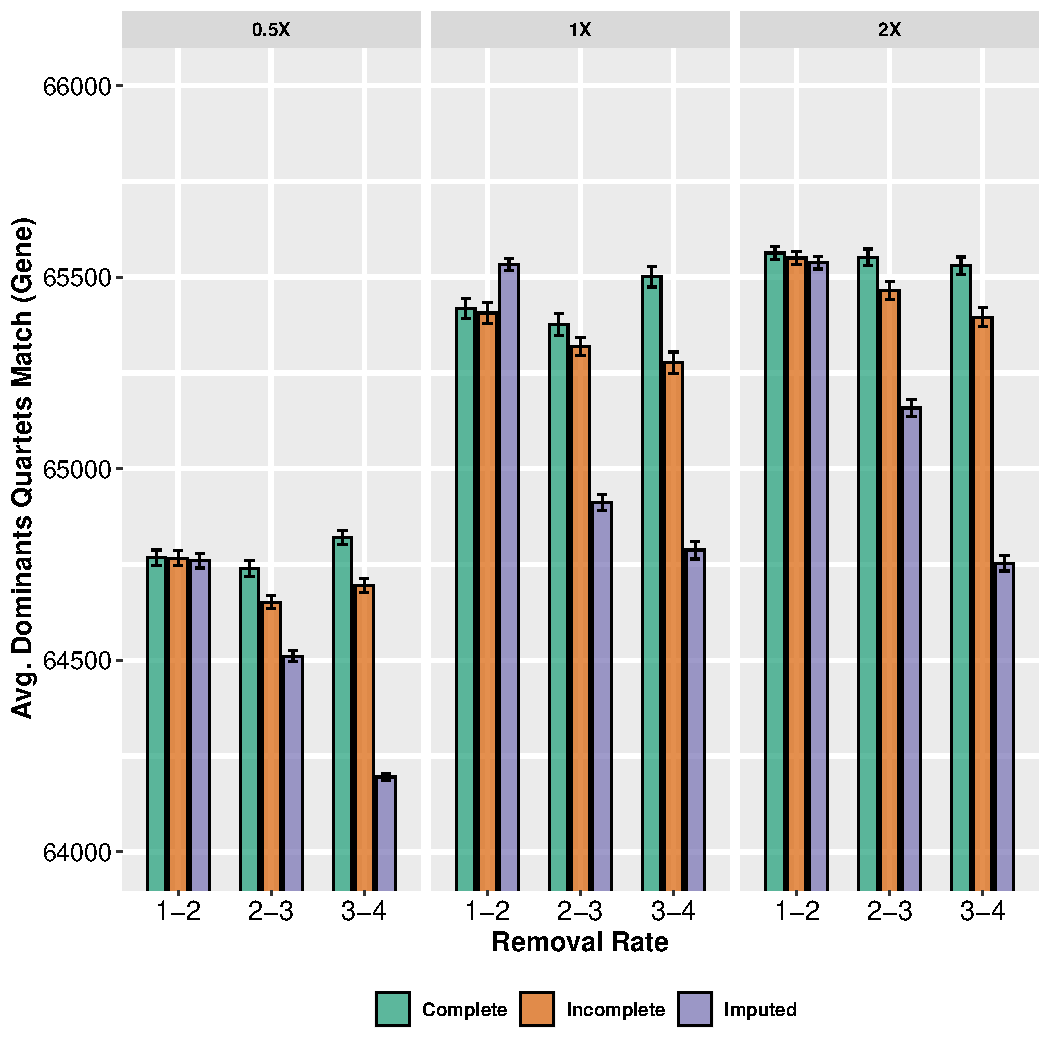
\includegraphics[width=\linewidth]{37_Taxon_Dataset/plot_QM.pdf}
%     \caption{The Quartet Matching between the quartet distributions of true gene trees and the complete, incomplete and the imputed gene trees for three taxa removal rate  i.e. 1-2, 2-3 and 3-4 taxa respectively.}
%     \label{fig:QM_37_taxon}
% \end{figure}


% \begin{figure}[H]
%     \centering
%     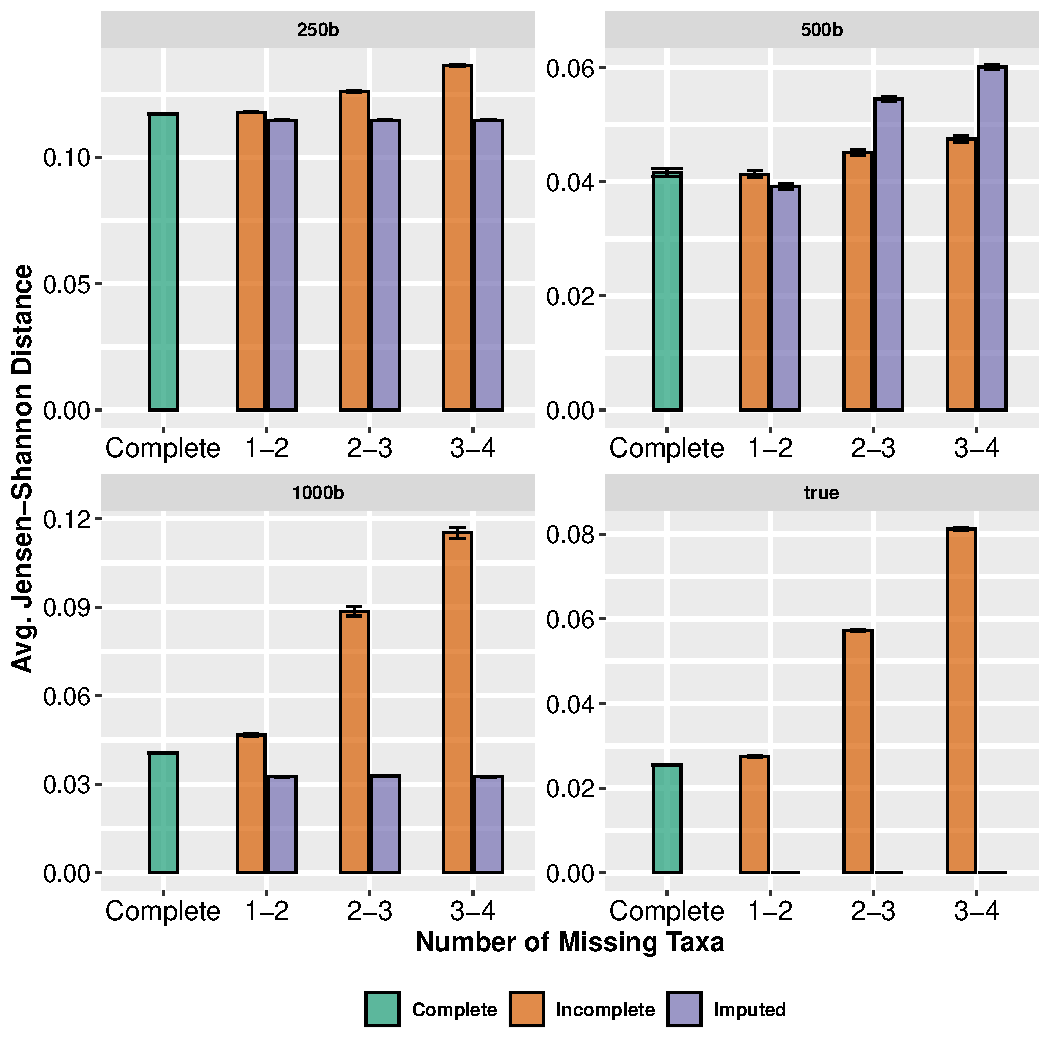
\includegraphics[width=\linewidth]{37_Taxon_Dataset/SequenceLength/plot_JSD_Gene.pdf}
%     \caption{The Jensen-Shannon Distance between the quartet distributions of true gene trees and the complete, incomplete and the imputed gene trees for three taxa removal rate  i.e. 1-2, 2-3 and 3-4 taxa respectively.}
%     \label{fig:JSD_37_taxon_seq}
% \end{figure}